\chapter{\IfLanguageName{dutch}{Stand van zaken}{State of the art}}
\label{ch:stand-van-zaken}

% Tip: Begin elk hoofdstuk met een paragraaf inleiding die beschrijft hoe
% dit hoofdstuk past binnen het geheel van de bachelorproef. Geef in het
% bijzonder aan wat de link is met het vorige en volgende hoofdstuk.

% Pas na deze inleidende paragraaf komt de eerste sectiehoofding.

In dit onderdeel zal de werking worden uitgelegd van een chatbot. Er zullen ook enkele van de meest bekende frameworks vergeleken worden met mekaar.

\section{Chatbot}
\label{sec:Chatbot}

Een chatbot is software die gemaakt is voor het automatiseren van een bepaalde taak. Er kan met de chatbot geconverseerd worden via een gebruikersinterface. Deze chatbot heeft op zich toegang tot bepaalde data die toegankelijk is via een API zodat het deze kan leveren aan een bepaalde gebruiker die hier om vraagt.

De gebruikersinterfaces kunnen zich bevinden op Messenger, Skype, Slack, WhatsApp, enz. Ook Siri en Alexa zijn bots, ze variëren van een chatfunctie tot een spraakassistent. Het is de bedoeling dat de gebruiker een vraag intypt en de chatbot geeft daar zo een gepast mogelijk antwoord op. Een chatbot kan zelf ook altijd een vraag stellen, dat kan zijn voor de naam van de persoon te weten te komen, zodat deze bot persoonlijker kan antwoorden. Het kan ook zijn voor een quiz of iets dergelijks.

Met NLP en machinelearning is het mogelijk om mensentaal aan een chatbot aan te leren. Deze hebben een zeer grote rol bij het maken van zo een bot. ~\autocite{assaf2017}

\section{Soorten Chatbots}
\label{sec:Soorten Chatbots}

Chatbots kunnen onderverdeeld worden in verschillende categorieën.

\subsection{Rule-Bases Bots}
\label{Rule-Bases Bots}

Een rule-based bot is een geautomatiseerde bot die reageert op bepaalde acties en sleutelwoorden en worden vaak ingezet op gespecialiseerde taken. Eén van de talen van zo een bot is AIML (Artificial Intelligence Markup Language), dat is een taal gebaseerd op XML. Deze laat toe om ontwikkelaars regels op te stellen voor een bot die deze moet volgen. Het is onmogelijk om regels te schrijven voor elk mogelijk scenario. ~\autocite{Kumar2017}

\subsection{AI-bot}
\label{AI-bot}

Een AI-bot simuleert het gedrag van een mens. Deze bot zal de bekende Turing-test moeten doorstaan. Deze test is ontwikkeld door Alan Turing in 1950. Hierin wordt gekeken of een mens onderscheid kan maken tussen een echte mens en een computer.

Deze bots zijn getraind aan de hand van een bepaalde hoeveelheid vragen. Voor elke vraag vindt de bot het meest relevante antwoord van alle mogelijke antwoorden. Zulke bots moeten ook rekening houden met de spelling en zinsbouw. Eenmaal deze ook goed getraind zijn daarop, zijn ze veel beter dan een rule-based bot.

\subsection{Generalistische bot}
\label{Generalistische bot}

Deze bots gebruiken vooral data uit databases en zoekmachines maar kunnen de gebruiker ook koppelen aan diensten. Deze heeft geen specifieke taak maar kan op een grote selectie van vragen antwoorden. Eenmaal de gebruiker iets specifieker in detail wil gaan over een bepaald onderwerp, kan deze bot overgaan naar een specialisatiebot.

\subsection{Specialisatiebot}
\label{Specialisatiebot}

Een specialisatiebot biedt een gespecialiseerde taak aan, dit vaak in tegenstelling tot een generalistische bot. Deze bot is uitsluitend bedoeld voor een specifiekere taak.

Generalistische en specialisatiebots werken vaak samen. Meestal begint het bij een generalistische bot die nog niet specifiek op iets ingaat. Het eindigt dan met een specialisatiebot die dan dieper ingaat op wat er precies wil geweten worden.

\section{Natural Language Processing (NLP)}
\label{sec:Natural Language Processing}

Vroeger typten we enkel commando's om te communiceren met een computer. Nu wordt er geprobeerd om met menselijke taal te communiceren met een computer. Natural Language Processing is de techniek die wordt gebruikt om menselijke taal te begrijpen.

NLP wordt al bij vele alledaagse dingen gebruikt. Bij de spellingscontroles in een e-mail of in de officepakketten. Bij een chatbot is dit al wat gecompliceerder, daar moet ook gekeken worden naar wat de gebruiker exact bedoeld met zijn input, de juiste intentie eruit halen.

NLP in de Nederlandse taal staat nog maar in zijn beginschoenen en zullen in vergelijking met de Engelstalige versie veel minder goed functioneren. ~\autocite{Dave2018}

\section{Natural Language Understanding (NLU)}
\label{sec:Natural Language Understanding}

Natural Language Understanding is een onderdeel van Natural Language Processing. Het is een vitaal onderdeel van een succesvol NLP. NLU focust zich primair op wat een bepaalde input betekent. Een input kan een zin zijn, gewone tekst of spraak. ~\autocite{Margaret2018}

\section{Artificial intelligence}
\label{sec:Artificial intelligence}

Machine learning werkt zonder directe input van een mens. Het probeert op zichzelf om algoritmes te verbeteren. Een bepaald algoritme heeft een doel. Machine learning zal trachten het algoritme te perfectioneren zodat de uitkomsten van nieuwe input dichter en dichter bij dat doel zullen liggen.

\section{Intents en Entities}
\label{sec:IntentsEntiteiten}

Als de gebruiker iets vraagt aan een chatbot is het doel van zijn vraag de intent, wat dus de intentie is van die vraag. Een intent kan ook entiteiten bevatten. Entiteiten zijn details van een intent. Als de gebruiker bijvoorbeeld vraagt aan de chatbot voor een vlucht te boeken, is de bestemming een entiteit.

\section{Feedback loops}
\label{sec:Feedback loops}

Wanneer een bepaalde input van een gebruiker nog niet is opgenomen in het machine learning algoritme van de chatbot is het de bedoeling dat aan de hand van deze feedback loops deze input op een automatische manier wordt gelinkt met de juiste intent en deze ongetrainde input te gebruiken voor de chatbot verder te trainen en deze slimmer te maken.

\section{Framework}
\label{sec:Framework}

Vandaag de dag bestaan er al veel API's die ontwikkelaars kunnen gebruiken voor AI/NLP-services. Zelfs zonder veel kennis van deze, kunnen ze makkelijk worden gebruikt. Luis.ai, Wit.ai zijn enkele voorbeelden van deze frameworks.

\section{Luis.ai}
\label{sec:Luis.ai}

\begin{figure}[h!]
	\centering
	
\includegraphics[height=2cm]{luis.png}
	\caption{Logo Luis.ai ~\autocite{Kevin2017}}
	\label{fig:luis}
\end{figure}
%Figure \ref{fig:luis} shows a logo.

Language Understanding (LUIS) is een op cloud gebaseerde API-service van microsoft voor het bepalen van de intentie van een gebruiker.  De input van een bepaalde gebruiker wordt via een Luis endpoint API verwerkt en krijgt daarop een gepast resultaat terug. De REST API van Luis kan gebruikt worden bij elk product, framework of service dat gebruik maakt van een HTTP request. ~\autocite{Dina2019}

\subsection{Verbeteren van de voorspellingen}
\label{verbeteren}

Nadat een Luis model is gepubliceerd en input ontvangt, zijn er enkele methodes voorzien om het model te verbeteren.

De eerste methode is aan de hand van patronen. Deze zorgen voor betere accuraatheid zonder veel meer voorbeeldzinnen te hoeven toevoegen. In de voorbeeldzinnen staan veel synoniemen, verschillende lengtes van zinnen, verschillende woordvolgordes, enz. Een patroon kan de woordvolgorde veel beter begrijpen.

De volgende methode werkt met woordengroeplijsten. Zo een lijst somt de woorden of zinnen op die verwant zijn met de applicatie. Wat LUIS dan leert over één van die woorden in een lijst, wordt automatisch toegepast op die andere woorden of zinnen in die bepaalde lijst. Het doel is voor het verbeteren van het identificeren van de juiste intent en entiteiten.

Er zijn 2 soorten types van lijsten. Een Interchangeable lijst is voor waarden die synoniemen zijn van mekaar. Een Non-interchangeable lijst is voor waarden die belangrijker zijn dan normale woorden. Dit helpt veel voor het bepalen van de juiste intent. Een Non-interchangeable lijst wordt ook gebruikt voor woorden die niet veel gebruikt worden of voor woorden of zinnen uit een andere taal, zo leert Luis rekening te houden met deze. Hierin bevinden zich meer de termen specifiek aan de applicatie. Bijvoorbeeld als de applicatie zal gaan over winkelen zullen er bepaalde termen gaande over winkelen zeer belangrijk zijn voor de app maar geen synoniemen zijn van mekaar.

De laatste methode voor het verbeteren van de voorspellingen is het actieve bijleren van de bot. Luis selecteert hier inputs die hij niet zeker van is wat de juiste intent is en zet deze in een lijst. De bedoeling is dat deze gevalideerd en gekoppeld worden aan de juiste intent met de juiste entiteiten. Dit moet echter manueel gebeuren door de eigenaar van de applicatie. Als deze inputs allemaal gelinkt zijn aan de juiste intent kan het model opnieuw getraind worden.

Luis plaatst inputs op de lijst waarvan hij helemaal niet zeker is waarbij deze behoort of waarbij hij twijfelt tussen twee of meerdere intents.

Het doel van dit onderzoek is om een manier te vinden om de inputs op deze lijst niet 100\% handmatig te moeten linken aan de juiste intent.

\section{Wit.ai}
\label{sec:Wit.ai}

\begin{figure}[h!]
	\centering
	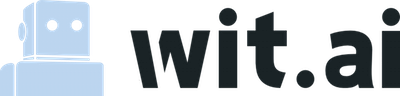
\includegraphics[height=2cm]{wit.png}
	\caption{Logo Wit.ai ~\autocite{Eva2016}}
	\label{fig:wit}
\end{figure}

Dit botframework is ontwikkeld door facebook. Wit helpt de gebruikers die iets zeggen tegen de chatbot van de app te verstaan. Wit dient ingesteld te worden door voorbeelden van zinnen toe te voegen net zoals Luis. Hoe meer voorbeelden er worden gegeven, hoe beter de bot de gebruikers zal begrijpen. De verzameling van voorbeeldzinnen voor 1 bepaalde intentie wordt dan gekoppeld aan de juiste intent. Er kan gemakkelijk gepraat worden met Wit via de endpoint API. 

Net zoals bij Luis is er een inbox met zinnen die zijn ingegeven door een gebruiker in de chatbot zelf die manueel moeten gelinkt worden aan de juiste intent. Wit stelt zelf al voor bij welke intent hij een bepaalde zin zou plaatsen. Deze kan aangepast worden indien deze fout is en de zinnen valideren. Deze worden dan opgenomen in het model als deze opnieuw wordt getraind. Ook dit deel zoals in Luis zou moeten kunnen gedeeltelijk geautomatiseerd worden. ~\autocite{Wit2019}

\section{API}
\label{sec:API}

Via een application programming interface (API) kan een programma communiceren met een ander programma of onderdeel hiervan. Bij een chatbot is het de bedoeling dat we in de applicatie die we ontwikkelen toegang krijgen tot de componenten van de chatbot. Zo kan er via het endpoint API van Luis of Wit de juiste intent uit een zin worden gehaald door de API aan te spreken. 

Naar mate van toegankelijkheid van de API van deze platformen zal er moeten gekeken worden of het mogelijk is om de inputs op te halen waar de bot aan twijfelt en deze automatisch te linken aan de juiste intent en deze inputs weer door te sturen naar het platform en zo linken aan de juiste intent zodat het model opnieuw kan worden getraind. ~\autocite{Kristian2011}     

%\section{State-of-the-art}
%\label{sec:state-of-the-art}

%\subsection{Chatbots}
%\label{Chatbots}

%\textcite{Knuth1998}
%~\autocite{Creeger2009}.
